\begin{document}
The current driver for this lab was created using an MCP6004 op amp. The op amp is to act as the driver for the gate of a 2N3904 Bipolar Junction Transistor (BJT). The generic circuit for the signal conditioner is shown in Figure \ref{fig:currentgeneric}. 
	
	\begin{figure}[H]
		\centering
		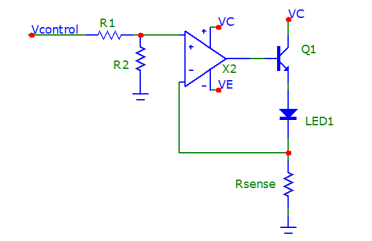
\includegraphics[width=.6\textwidth]{CircuitDevelopment/ledgeneric.png}
		\caption{Generic current driver circuit \cite{b2}}
		\label{fig:currentgeneric}
	\end{figure}

The key to operation of the current driver is the BJT transistor. A BJT transistor, in contrast with the metal oxide semiconducting field effect transistor (MOSFET), is capable of 


\end{document}